\documentclass[tikz,border=12pt]{standalone}
\usepackage[T1]{fontenc}
\usepackage{lmodern}
\usetikzlibrary{backgrounds,calc,positioning}

\definecolor{docblue}{HTML}{1565C0}
\definecolor{chunkteal}{HTML}{00838F}
\definecolor{summaryorange}{HTML}{E65100}
\definecolor{combinegreen}{HTML}{2E7D32}
\definecolor{answergreen}{HTML}{1B5E20}
\definecolor{softgray}{HTML}{ECEFF1}
\definecolor{textgray}{HTML}{455A64}

\newcommand{\flowband}[7]{%
  \path[fill=#7, draw=black!18, line width=0.35pt]
    (#1,#2) .. controls (#1 + 1.1,#2) and (#4 - 1.1,#5) .. (#4,#5)
    -- (#4,#6)
    .. controls (#4 - 1.1,#6) and (#1 + 1.1,#3) .. (#1,#3)
    -- cycle;
}

\begin{document}
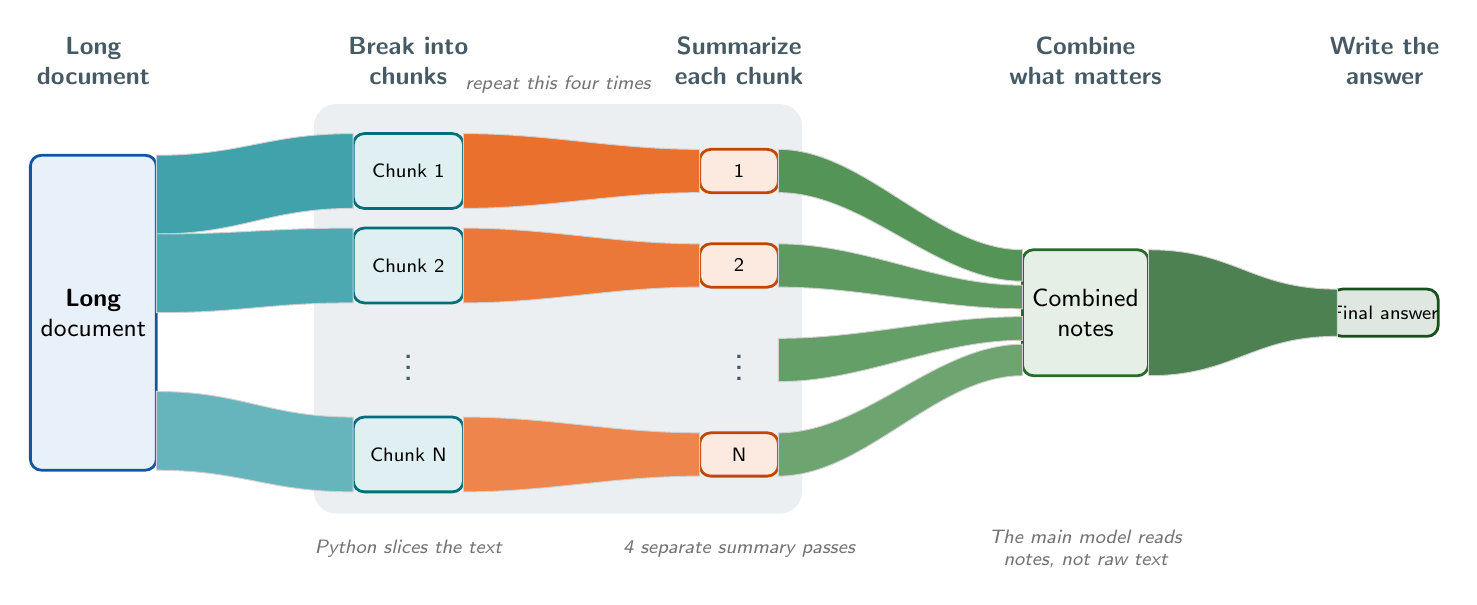
\begin{tikzpicture}[
		font=\sffamily\small,
		stage/.style={font=\sffamily\bfseries\small, align=center, text=textgray},
		note/.style={font=\sffamily\scriptsize\itshape, align=center, text=black!55},
		box/.style={rounded corners=4pt, line width=1pt, align=center, inner sep=0pt},
	]

	% x coordinates
	\def\xdoc{0.0}
	\def\xchunk{4.0}
	\def\xsummary{8.2}
	\def\xcombine{12.6}
	\def\xanswer{16.4}

	% visible node geometry
	\def\docw{1.6}
	\def\doch{4.0}
	\def\chunkw{1.4}
	\def\chunkh{0.95}
	\def\sumw{1.0}
	\def\sumh{0.55}
	\def\combw{1.6}
	\def\combh{1.6}
	\def\answ{1.2}
	\def\ansh{0.60}

	% right/left edges used for flow bands
	\pgfmathsetmacro{\docright}{\xdoc + 0.5*\docw}
	\pgfmathsetmacro{\chunkleft}{\xchunk - 0.5*\chunkw}
	\pgfmathsetmacro{\chunkright}{\xchunk + 0.5*\chunkw}
	\pgfmathsetmacro{\sumleft}{\xsummary - 0.5*\sumw}
	\pgfmathsetmacro{\sumright}{\xsummary + 0.5*\sumw}
	\pgfmathsetmacro{\combineleft}{\xcombine - 0.5*\combw}
	\pgfmathsetmacro{\combineright}{\xcombine + 0.5*\combw}
	\pgfmathsetmacro{\answerleft}{\xanswer - 0.5*\answ}

	% stage labels
	\node[stage] at (\xdoc, 3.2) {Long\\document};
	\node[stage] at (\xchunk, 3.2) {Break into\\chunks};
	\node[stage] at (\xsummary, 3.2) {Summarize\\each chunk};
	\node[stage] at (\xcombine, 3.2) {Combine\\what matters};
	\node[stage] at (\xanswer, 3.2) {Write the\\answer};

	% notes
	\node[note] at (\xchunk, -3.0) {Python slices the text};
	\node[note] at (\xsummary, -3.0) {4 separate summary passes};
	\node[note] at (\xcombine, -3.0) {The main model reads\\notes, not raw text};

	% visible nodes
	\node[box, draw=docblue!85!black, fill=docblue!10,
		minimum width=\docw cm, minimum height=\doch cm] (doc) at (\xdoc, 0)
	{\textbf{Long}\\document};

	\node[box, draw=chunkteal!85!black, fill=chunkteal!12,
		minimum width=\chunkw cm, minimum height=\chunkh cm,
		font=\sffamily\scriptsize] (chunk1) at (\xchunk, 1.8) {Chunk 1};
	\node[box, draw=chunkteal!85!black, fill=chunkteal!12,
		minimum width=\chunkw cm, minimum height=\chunkh cm,
		font=\sffamily\scriptsize] (chunk2) at (\xchunk, 0.6) {Chunk 2};
	\node[font=\sffamily\Large, text=textgray] (chunk3) at (\xchunk, -0.6) {\vdots};
	\node[box, draw=chunkteal!85!black, fill=chunkteal!12,
		minimum width=\chunkw cm, minimum height=\chunkh cm,
		font=\sffamily\scriptsize] (chunk4) at (\xchunk, -1.8) {Chunk N};

	\node[box, draw=summaryorange!85!black, fill=summaryorange!12,
		minimum width=\sumw cm, minimum height=\sumh cm,
		font=\sffamily\scriptsize] (sum1) at (\xsummary, 1.8) {1};
	\node[box, draw=summaryorange!85!black, fill=summaryorange!12,
		minimum width=\sumw cm, minimum height=\sumh cm,
		font=\sffamily\scriptsize] (sum2) at (\xsummary, 0.6) {2};
	\node[font=\sffamily\Large, text=textgray] (sum3) at (\xsummary, -0.6) {\vdots};
	\node[box, draw=summaryorange!85!black, fill=summaryorange!12,
		minimum width=\sumw cm, minimum height=\sumh cm,
		font=\sffamily\scriptsize] (sum4) at (\xsummary, -1.8) {N};

	\node[box, draw=combinegreen!85!black, fill=combinegreen!12,
		minimum width=\combw cm, minimum height=\combh cm] (combine) at (\xcombine, 0)
	{Combined\\notes};

	\node[box, draw=answergreen!85!black, fill=answergreen!14,
		minimum width=\answ cm, minimum height=\ansh cm,
		font=\sffamily\scriptsize] (answer) at (\xanswer, 0)
	{Final answer};

	% document -> chunks
	\flowband{\docright}{2.0}{1.0}{\chunkleft}{2.275}{1.325}{chunkteal!75}
	\flowband{\docright}{1.0}{0.0}{\chunkleft}{1.075}{0.125}{chunkteal!70}
	\flowband{\docright}{-1.0}{-2.0}{\chunkleft}{-1.325}{-2.275}{chunkteal!60}

	% chunks -> summaries (narrower bands show compression)
	\flowband{\chunkright}{2.275}{1.325}{\sumleft}{2.075}{1.525}{summaryorange!82}
	\flowband{\chunkright}{1.075}{0.125}{\sumleft}{0.875}{0.325}{summaryorange!78}
	\flowband{\chunkright}{-1.325}{-2.275}{\sumleft}{-1.525}{-2.075}{summaryorange!70}

	% summaries -> combined notes
	\flowband{\sumright}{2.075}{1.525}{\combineleft}{0.80}{0.40}{combinegreen!82}
	\flowband{\sumright}{0.875}{0.325}{\combineleft}{0.35}{0.05}{combinegreen!78}
	\flowband{\sumright}{-0.325}{-0.875}{\combineleft}{-0.05}{-0.35}{combinegreen!74}
	\flowband{\sumright}{-1.525}{-2.075}{\combineleft}{-0.40}{-0.80}{combinegreen!70}

	% combined notes -> answer
	\flowband{\combineright}{0.80}{-0.80}{\answerleft}{0.30}{-0.30}{answergreen!78}

	% soft guide behind the repeated middle steps
	\begin{scope}[on background layer]
		\fill[softgray, rounded corners=8pt]
		(2.8, 2.65) rectangle (9.0, -2.55);
	\end{scope}

	\node[note] at (5.9, 2.9) {repeat this four times};

\end{tikzpicture}
\end{document}
